The intial visualization of the light curve was further analyzed to idnetify and quatify key 
features of the curve. Using Python, the script calculated the average flux level and identified 
the minimum flux point, showing the center of the primary eclipse. This point occurred at 
approximately HJD 2460634.67.

Measuring the eclipse depth, the difference between the maximum and minimum relative flux was also
computed. The depth was found to be about 0.032, showing a significant contrast in brightness 
during the eclipse. Secondly, the duration of the eclipse was estimated by identifying the time
range in which the flux was below the average. The calculated duration was about 0.038 days (or about 55 minutes.

Figure~\ref{fig:analyzedcurve} illustrated the annotated light curve with the mean flux, 
minimum flux, and eclipsing event clearly marked. This figure highlights the This graphic 
demonstrates how well photometric analysis works to identify important physical characteristics of 
eclipsing binary systems.

The intrinsic brightness of the system was computed using the inverse-square law in order to further 
interpret the flux data in a physically meaningful manner. For every data point, the brightness was 
calculated using the known distance of 34.13 light-years. This change is visualzied in
Figure~\ref{fig:luminositycurve}, which shows the variation in luminosity over time, corresponding
to the change in flux over time.

\begin{figure}[h!]
	\centering
	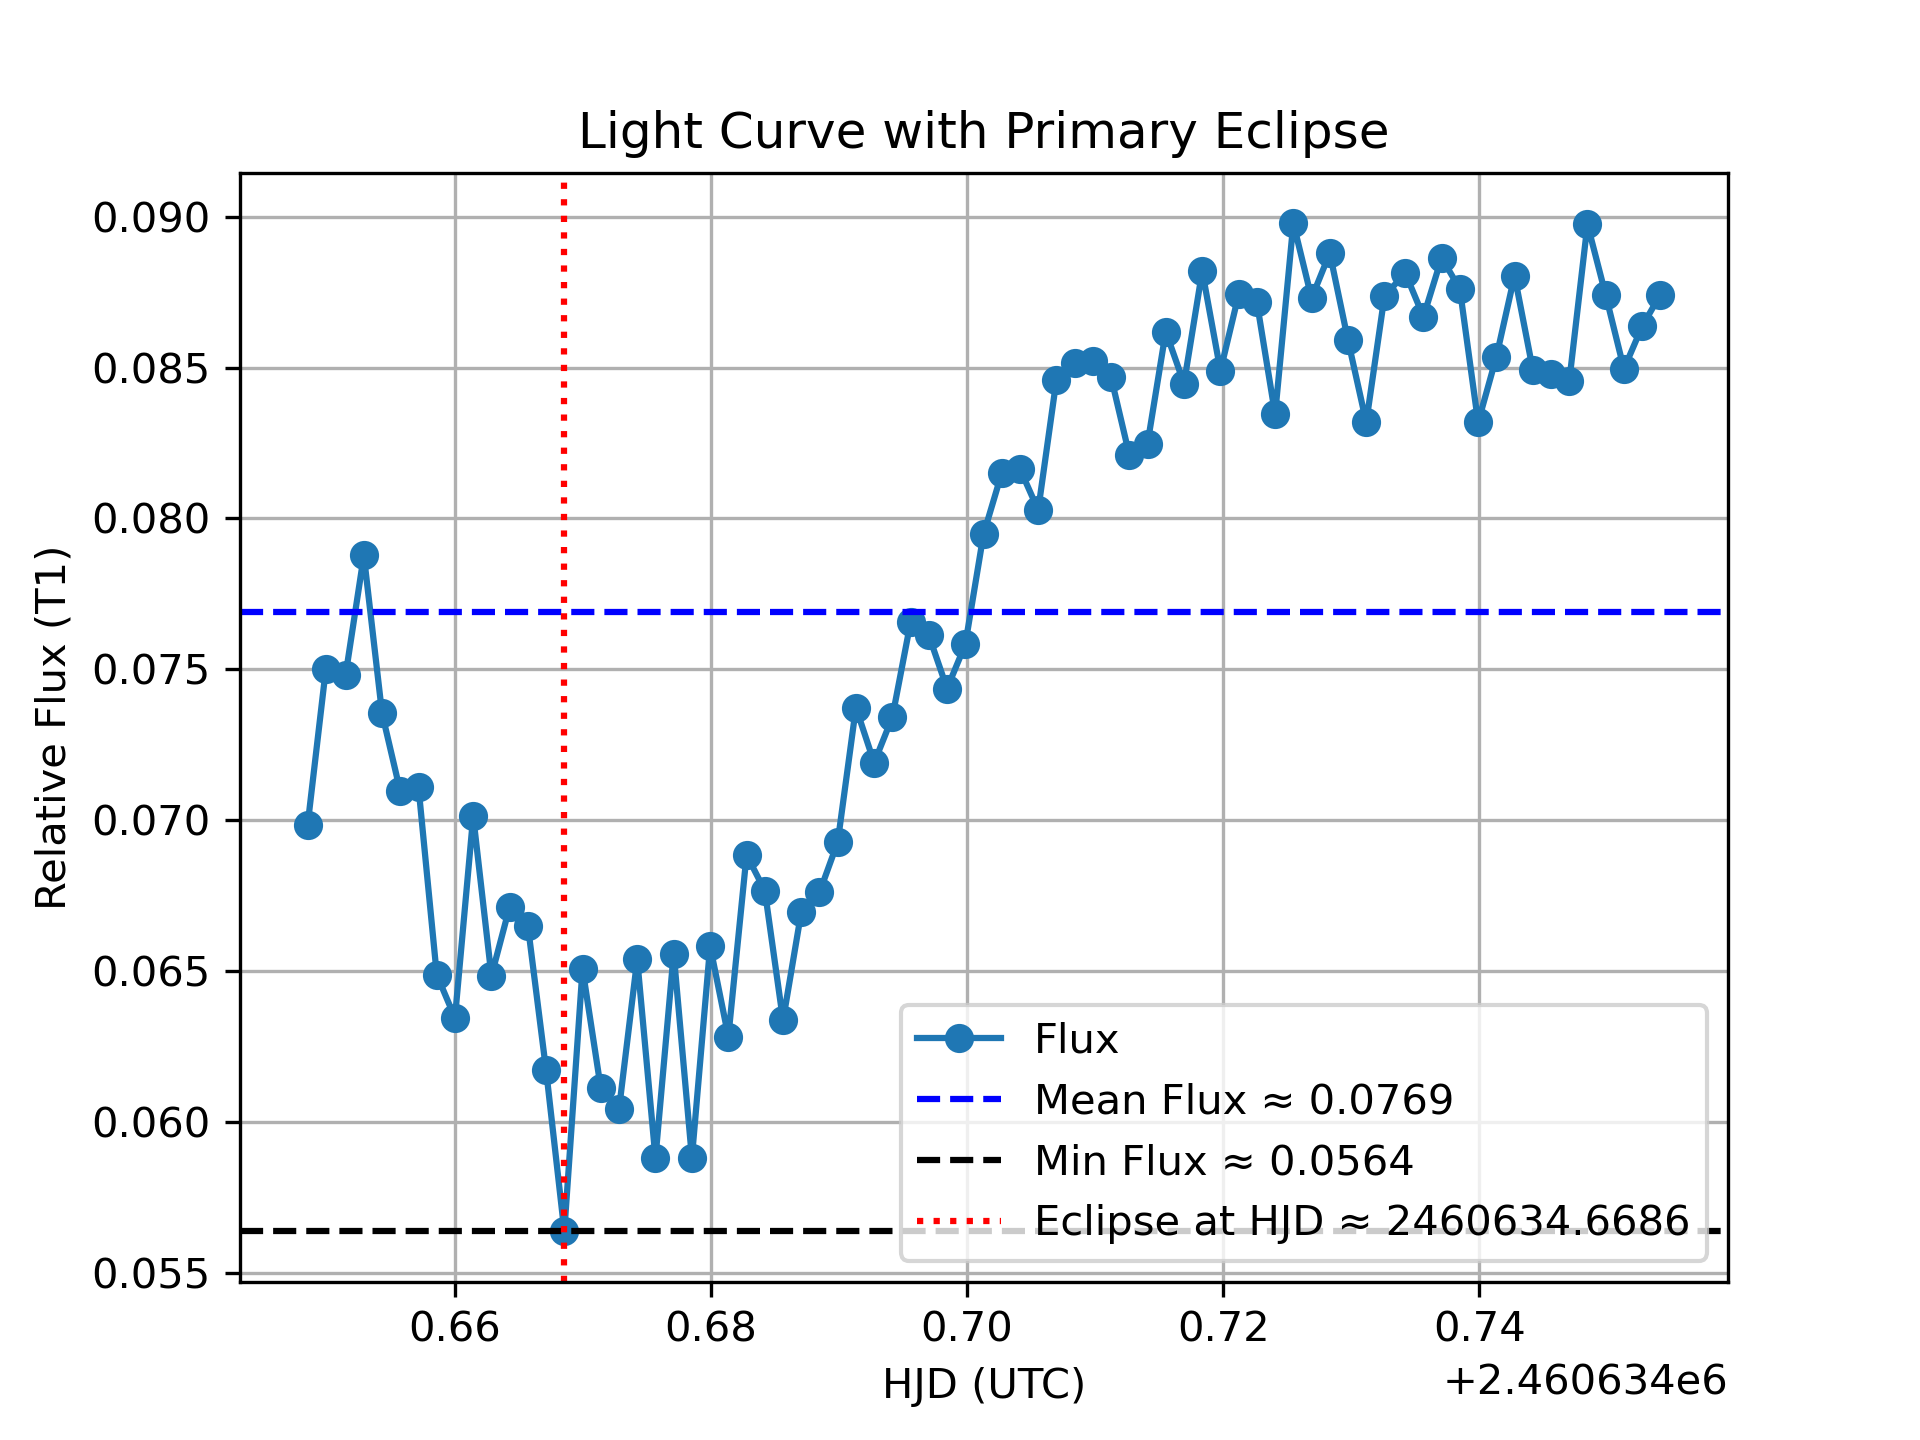
\includegraphics[width=0.8\textwidth]{figs/analyzed_light_curve.png}
	\caption{Analyzed light curve showing mean flux, minimum flux, and estimated duration}
	\label{fig:analyzedcurve}
\end{figure}

\begin{figure}[h!]
        \centering
        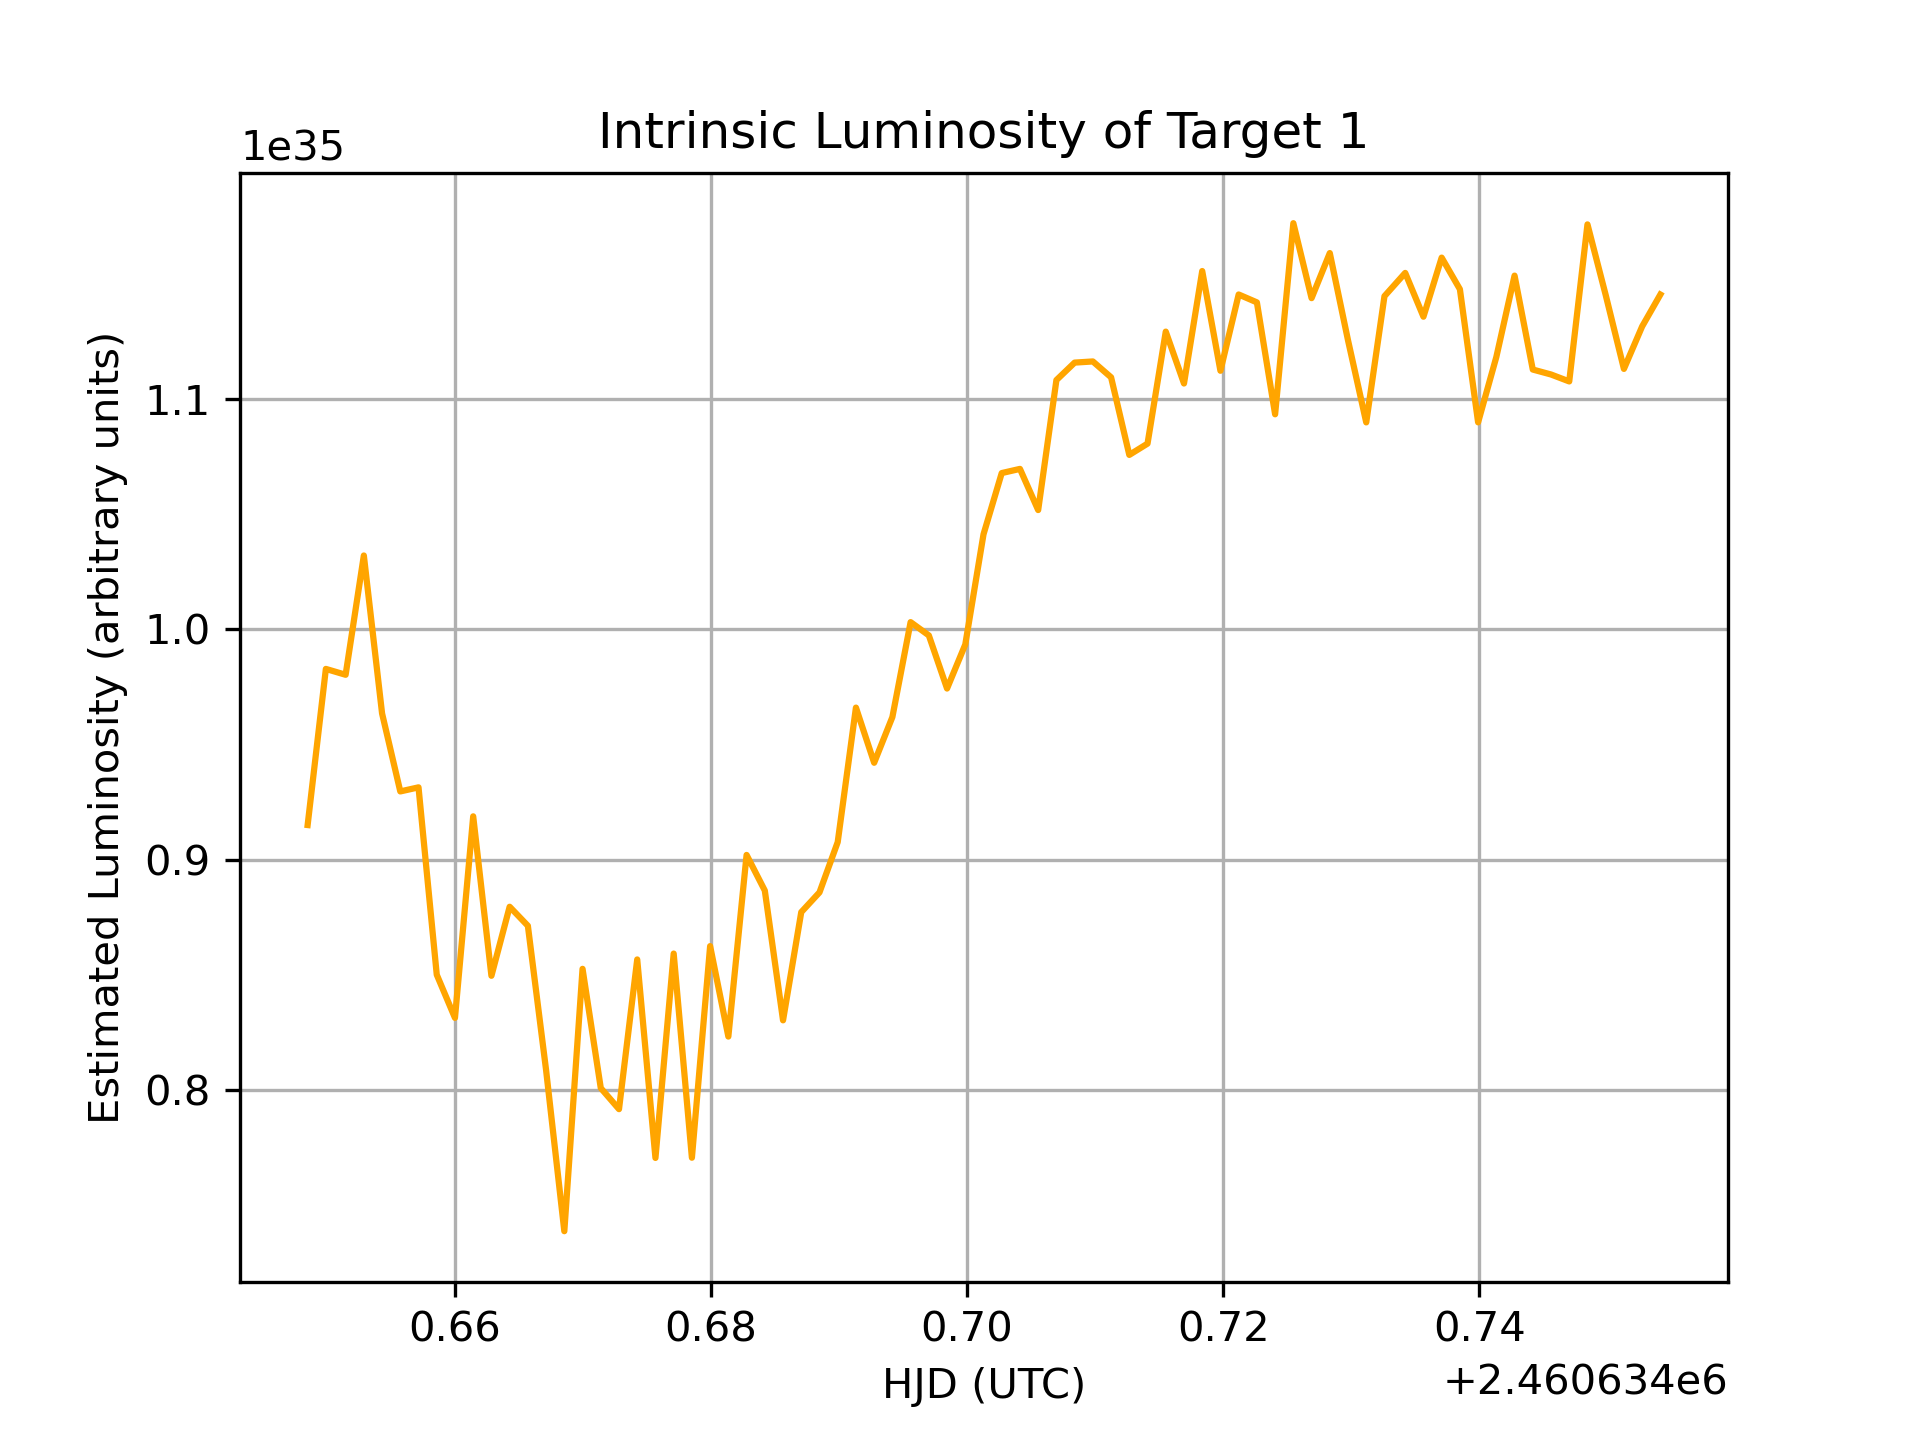
\includegraphics[width=0.8\textwidth]{figs/luminosity_curve.png}
        \caption{Intrinsic luminosity of the system calculated using inverse-square law and known distance of 34.14 light years.}
        \label{fig:luminositycurve}
\end{figure}
